\documentclass[12pt,a4paper]{article}

\usepackage[utf8]{inputenc}
\usepackage[english]{babel}
\usepackage{amsmath}
\usepackage{amsfonts}
\usepackage{amssymb}
\usepackage{graphicx}
\usepackage{cite}
\usepackage{hyperref}
\usepackage[left=2cm,right=2cm,top=2cm,bottom=2cm]{geometry}
\usepackage{booktabs}
\usepackage{xcolor,colortbl}
\usepackage{pstricks}
\usepackage{eurosym} 
\usepackage{longtable}
\usepackage{blindtext}
\usepackage{fancyhdr}
\usepackage{lastpage}
\usepackage{pdfpages}
\usepackage{tabularx} 
\usepackage{transparent}
\usepackage{array}
\usepackage{etoolbox}
\usepackage{float}
\usepackage{lscape}

\author{Communications Department}
\title{Communications. Physical Network Topology}


\begin{document}
\section{Aim of the document}
This document has been created in order to take a decision about the physical topology of our satellite's network and also to decide if we want or need global coverage or not. It is a very important decision due to the fact that reliability, performance and security are related with the physical topology. The most usual are: 
\begin{itemize}
\item Mesh
\item Star
\item Bus
\item Ring
\item Hybrid
\end{itemize}
In the following section the members of the groups will explain what they think the best option is, giving reasons for and against that decision. 
	% PROPUESTA BOYAN
	\section{Propuesta Boyan}
	\paragraph{}
	Options:
	\begin{itemize}
		\item Ideal case scenario: Global Coverage with lowest possible orbit.
	\item Not so ideal case scenario: Global Coverage with some satellites in a higher orbit acting as a hub.
	\end{itemize}
After reviewing \cite{Wood1998}, \cite{Muri2012}, \cite{Horne2002}, \cite{Wood2001}, \cite{BookchapterinServiceEfficientNetworkInterconnectionviaSatellite2002}, 
\cite{Goodwin1998}, \cite{Sun2015} and \cite{Baumann} my proposal is the next:
\newline

·Use of the \textbf{Manhattan Topology} for our constellation, mixed with a \textit{Walker Delta} or a \textit{Walker Polar} orbits configuration.
\\

%ISL can be very high, with  very high data rates and then, sat to ground can be lower but we can divide it through the network

\textit{"The Manhattan network is the underlying form of the ISL satellite constellation’s
network topology. This is a regular topology named after the regular grid street
pattern established in Manhattan Island, New York. It is a toroidal mesh network with
each node having four unidirectional links: two transmit and two receive
[Maxemchuk87], as shown in figure 2.9.
Manhattan networks have been extensively discussed in computing literature in the
context of parallel computing. The Manhattan network forms the basic topology of the
type (2) constellation. The Manhattan network is also known as a multiaccess mesh or
multimesh network [ToddHahne97]. The form of the Manhattan network with bidirectional
links is known as either the bi-directional Manhattan network, as the HR4-
net [ChungSharAg94], or as the shufflenet.
However, orbital geometry leads to differences from previously discussed Manhattan networks. In fact, the constellation network is a slightly variant form, with bidirectional
ISLs and with two half-twists where the sense of rotation changes due to
each satellite seeing its neighbours swap sides while ‘down’ remains constant as the
satellites reach and pass through their highest latitudes. The topologies of the space
segments of Iridium, Teledesic, and Spaceway NGSO can be considered as variations
on the type of bi-directional Manhattan network shown in figure 2.10."}\cite[p. 32]{Wood2001} \textbf{(en Mendeley)}

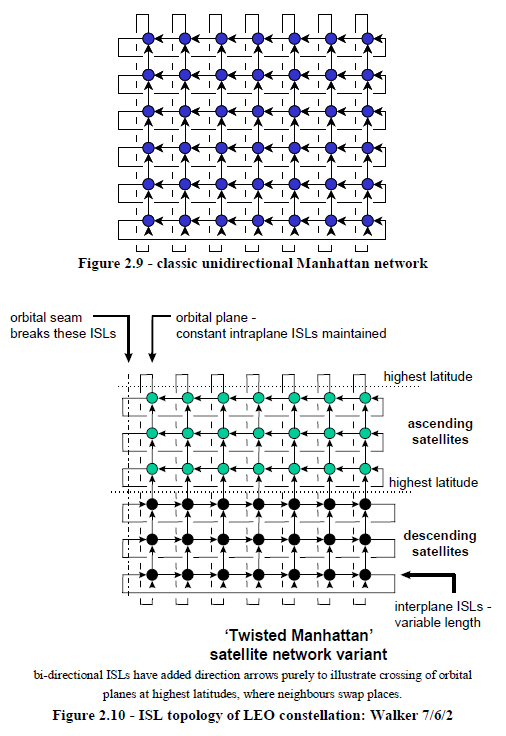
\includegraphics[scale=1]{parts/W_D}

	%Propuesta Eva 
	\section{Propuesta Eva}

	%Propuesta Josep
	\section{Propuesta Josep}
\subsection{Coverage}
I hold the view that we should offer as much coverage as possible, ideally full coverage, so that the range of clients is as broad as possible. So if it is technically feasible, I think we should intend to create a full coverage network. I agree with Eva, we do not need to create Ground Stations all around the world, it is responsability of the client, which is supposed to be a professional of the field, and therefore would have a proper Ground Station, hardware and knowledge to use and dominate it.
\subsection{Physical topology}
As it has been already said before, both mesh and star topology do not match our requirements. The option that Boyan has suggested (The Manhattan Topology) seems pretty nice, but Eva's suggestion too. In fact, they seem to be a bit similar. This seems a good direction to take. We should decide further details and maybe solve some little problems, but this is the kind of topology that I would take too. We should take into account the fact that distance between satellites might change, and be sure that in the furthest point, the communication is acceptable. We should also consider effects such as Doppler Effect (both the transmitter and the receiver are moving). This requires a further study, but this is the direction that I would definitely take. It would be nice if we could discuss it via Skype or any other communication programme, and decide exactly if Boyan's or Eva's option (though quite similar, a few differences exist).


	%Propuesta Josep Maria
	\section{Josep Maria Proposal}

\subsection{Requirements}

\paragraph{} First of all, we must take into account the requirements of our constellation. Those requirements are the following:
\pagebreak
\begin{table}[htb]
\centering
\begin{tabular}{c p{14cm}}
\toprule
\textbf{Feature} & \textbf{Description}                                                                                                                                                          \\ \midrule
1                & \begin{tabular}[c]{@{}l@{}}Provide communication relay between two LEO nanosatellites with a latency \\ \textbf{lower than 1 minute}.\end{tabular}\vspace{0.3cm}                                                 \\
2                & \begin{tabular}[c]{@{}l@{}}Provide communication relay between a LEO nanosatellite and the ground \\ with a latency \textbf{lower than 5 minutes.}.\end{tabular}\vspace{0.3cm}                                                                                        \\
3                & \begin{tabular}[c]{@{}l@{}}Back-up system prepared to handle \textbf{up to two major failures} in the system.\\ A major failure can be defined as the loss of a client’s satellite coverage because\\ of a failure in the network.\end{tabular}\vspace{0.3cm}                                                 \\
4                & \begin{tabular}[c]{@{}l@{}}Switch time after major failure happens, shall be\textbf{ below 6 hours}.\end{tabular}\vspace{0.3cm}                                                                                                     \\
5                & \begin{tabular}[c]{@{}l@{}}Each Satellite Node volume should be equal or \textbf{lower than a 3U Cubesat.}\end{tabular}\vspace{0.3cm}                                                                                                     \\
6                & \begin{tabular}[c]{@{}l@{}}Each Node should be able to handle \textbf{at least 25 Mbit/s} of data rate.\end{tabular}\vspace{0.3cm}                                                                                                     \\ \bottomrule
\end{tabular}
\caption{Project Requirements}
\end{table}

\paragraph{}The most restricting requirements are:

\begin{itemize}
\item Back-up system prepared to handle \textbf{up to two major failures} in the system.
\item Switch time after major failure happens, shall be\textbf{ below 6 hours}.
\end{itemize}

\paragraph{}This requirements limit the type of network architecture that can be implemented. A ring network will fail completely if two major failures isolate one segment from the rest of the ring. A star network will fail if the hub has a major failure. It has to be taken into account that 6 hours is not enough time to replace a satellite node. A full mesh network will simply not work because not all satellites are visible due to the Earth being in the middle of the constellation. This only leaves us with different kinds of hybrid networks. The proposal in this section is the implementation of a mesh-ring hybrid network.


\subsection{Network}

\paragraph{}For this proposal to be effective, the satellite constellation has to be done in a series of polar, or near polar, orbits where all planes move in the same direction. This will create two hemispheres where in one the satellites move from south to north, and in the other one they move from north to south. If there were two adjacent planes moving in opposite directions, the relative velocity of the satellites will be very high, and its relative position will also vary significantly, almost covering 180º. Aside from Doppler effects, this configuration will need a tracking system for two antennas or invest a lot of power in a antenna with very wide range, and since our satellites are cubesats of 3 units at maximum, it is preferable to not have this kind of systems.

\paragraph{}With this configuration, the general idea is to design a network where each satellite node has a link with four neighbouring ones. Two of this links will be with the next and previous satellite of the same orbital plane. The other two will be with be with a satellite in the two adjacent planes, with the exception of the orbital planes which neighbours will move in the other direction (one plane moving north-to-south, and the adjacent moving south-to-north). This links between satellites can be bi-directional.

\begin{figure}[H]
\centering
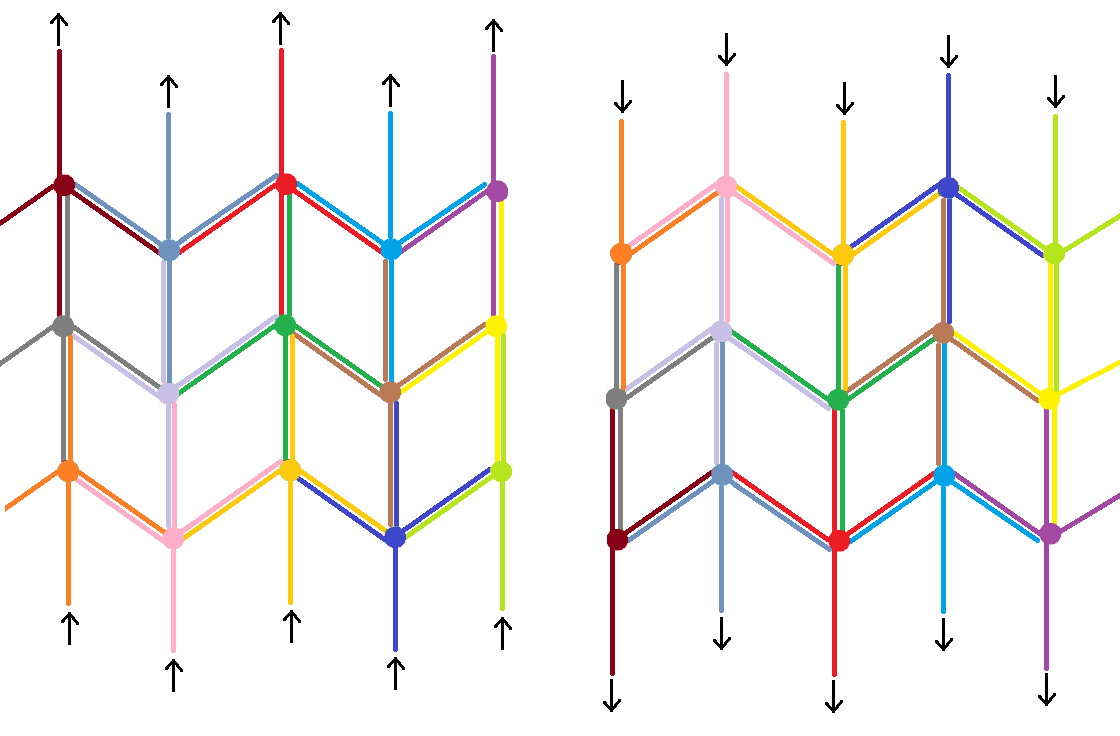
\includegraphics[scale=0.5]{./parts/img_jm/network}
\caption[Scheme of the topology]{Scheme of the topology of the network, where each dot is a satellite, each line a data link and the arrows indicate the direction that each orbital plane moves}
\label{Scheme of the topology}
\end{figure}

\paragraph{}The idea behind this configuration is that if a satellite node fails, the data has two more nodes to travel to. Since the position of the nodes in the same orbital plane do not vary relatively to a satellite in the same plane, the two links do not need to be very powerful, since the antenna range can be very narrow. The problem lies with tha two satellites in the adjacent planes, which position will vary relative to the satellite node. This will require two antennas with a range of 120º aproximately.
	
	
	
	
	% BIBLIOGRAPHY
	\bibliography{boyan,eva}{}
	\bibliographystyle{plain}
	
	
\end{document}
